%                      Code_Saturne version 1.3
%                      ------------------------
%
%     This file is part of the Code_Saturne Kernel, element of the
%     Code_Saturne CFD tool.
%
%     Copyright (C) 1998-2008 EDF S.A., France
%
%     contact: saturne-support@edf.fr
%
%     The Code_Saturne Kernel is free software; you can redistribute it
%     and/or modify it under the terms of the GNU General Public License
%     as published by the Free Software Foundation; either version 2 of
%     the License, or (at your option) any later version.
%
%     The Code_Saturne Kernel is distributed in the hope that it will be
%     useful, but WITHOUT ANY WARRANTY; without even the implied warranty
%     of MERCHANTABILITY or FITNESS FOR A PARTICULAR PURPOSE.  See the
%     GNU General Public License for more details.
%
%     You should have received a copy of the GNU General Public License
%     along with the Code_Saturne Kernel; if not, write to the
%     Free Software Foundation, Inc.,
%     51 Franklin St, Fifth Floor,
%     Boston, MA  02110-1301  USA
%
%-----------------------------------------------------------------------
%

\programme{clsyvt}

\vspace{1cm}
%%%%%%%%%%%%%%%%%%%%%%%%%%%%%%%%%%
%%%%%%%%%%%%%%%%%%%%%%%%%%%%%%%%%%
\section{Fonction}
%%%%%%%%%%%%%%%%%%%%%%%%%%%%%%%%%%
%%%%%%%%%%%%%%%%%%%%%%%%%%%%%%%%%%
Le but de ce sous-programme est de remplir les tableaux de conditions aux
limites (\var{COEFA} et \var{COEFB}) pour la vitesse et le tenseur de Reynolds,
pour les faces de sym\'etrie. Ces conditions s'\'ecrivent assez
naturellement dans le rep\`ere local \`a la face. La fonction de \fort{clsyvt}
est alors de partir de ces conditions naturelles dans rep\`ere local, de les
transformer dans le rep\`ere g\'en\'eral, et de les impliciter \'eventuellement
en partie.

On note que le sous-programme \fort{clptur} (pour les conditions aux parois)
contient une partie \'ecriture dans
le rep\`ere local et rotation totalement similaire.

%%%%%%%%%%%%%%%%%%%%%%%%%%%%%%%%%%
%%%%%%%%%%%%%%%%%%%%%%%%%%%%%%%%%%
\section{Discr\'etisation}
%%%%%%%%%%%%%%%%%%%%%%%%%%%%%%%%%%
%%%%%%%%%%%%%%%%%%%%%%%%%%%%%%%%%%

La figure \ref{Base_Clsyvt_fig_facesym} pr\'esente les notations utilis\'ees \`a la face. Le
rep\`ere local est d\'efini \`a partir de la normale \`a la face et la vitesse
en $I'$ :\\
$\bullet\ \displaystyle\vect{t}
=\frac{1}{|\vect{u}_{I',\tau}|}\vect{u}_{I',\tau}$ est le
premier vecteur du rep\`ere local.\\
$\bullet\ \vect{\tilde{n}}=-\vect{n}$ est le deuxi\`eme vecteur du rep\`ere
local.\\
$\bullet\ \vect{b}=\vect{t}\wedge\vect{\tilde{n}}=\vect{n}\wedge\vect{t}$ est le
troisi\`eme vecteur du rep\`ere local.

\begin{figure}[h]
\centerline{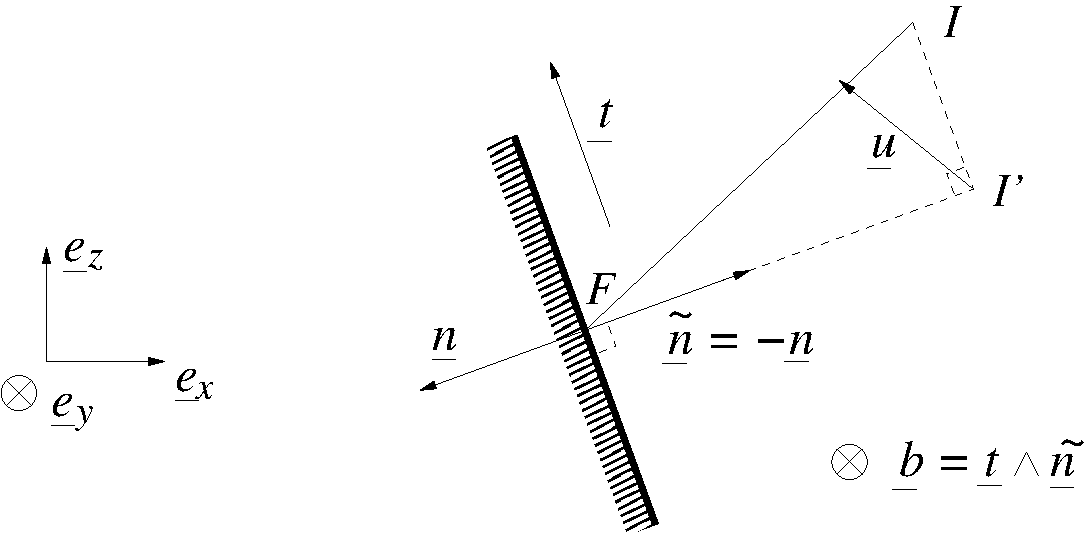
\includegraphics[width=8cm]{\repgraphics/facesym}}
\caption{\label{Base_Clsyvt_fig_facesym}D\'efinition des vecteurs de base du rep\`ere local}
\end{figure}

Ici, $\vect{n}$ est la normale \`a la face de bord au sens de \CS ({\em i.e.}
pointant vers l'ext\'erieur) et $\vect{u}_{I',\tau}$ est la projection de la
vitesse en $I'$ dans le plan de la face :
$\vect{u}_{I',\tau}=\vect{u}_{I'}-(\vect{u}_{I'}.\vect{n})\vect{n}$.\\
Si $\vect{u}_{I',\tau}=\vect{0}$, l'orientation de $\vect{t}$ dans le plan
normal \`a $\vect{n}$ est sans importance. On le d\'efinit alors par :
$\displaystyle\vect{t}=\frac{1}{\sqrt{n_y^2+n_z^2}}(n_z\vect{e}_y-n_y\vect{e}_z)$
ou
$\displaystyle\vect{t}=\frac{1}{\sqrt{n_x^2+n_z^2}}(n_z\vect{e}_x-n_x\vect{e}_z)$
suivant les composantes de $\vect{n}$ qui sont non nulles (composantes dans le
rep\`ere global $(\vect{e}_x,\vect{e}_y,\vect{e}_z)$).


Pour plus de clart\'e, on utilisera les notations suivantes :\\
$\bullet\ $Le rep\`ere g\'en\'eral sera not\'e
$\mathcal{R}=(\vect{e}_x,\vect{e}_y,\vect{e}_z)$.\\
$\bullet\ $Le rep\`ere local sera not\'e
$\hat{\mathcal{R}}=(\vect{t},-\vect{n},\vect{b})=(\vect{t},\vect{\tilde{n}},\vect{b})$.\\
$\bullet\ $Les matrices des composantes d'un vecteur $\vect{u}$ dans les rep\`eres
$\mathcal{R}$ et $\hat{\mathcal{R}}$ seront not\'ees respectivement
$\mat{U}$ et $\hat{\mat{U}}$.\\
$\bullet\ $Les matrices des composantes d'un tenseur $\tens{R}$ (d'ordre 2) dans
les rep\`eres $\mathcal{R}$ et $\hat{\mathcal{R}}$ seront not\'ees
respectivement $\matt{R}$ et $\hat{\matt{R}}$.\\
$\bullet\ $On note $\matt{P}$ la matrice (orthogonale) de passage de $\mathcal{R}$ \`a
$\hat{\mathcal{R}}$.
\begin{equation}
\matt{P}=\left[
\begin{array}{ccc}
t_x & -n_x & b_x\\
t_y & -n_y & b_y\\
t_z & -n_z & b_z
\end{array}\right]
\end{equation}

($\matt{P}$ \'etant orthogonale, $\matt{P}^{-1}=\,^t\matt{P}$).

On a alors en particulier les relations suivantes, pour tout vecteur $\vect{u}$
et tout tenseur $\tens{R}$ d'ordre 2 :\\
\begin{equation}
\left\{\begin{array}{l}
\mat{U} = \matt{P}\,.\,\hat{\mat{U}}\\
\matt{R}= \matt{P}\,.\,\hat{\matt{R}}\,.\,^t\matt{P}
\end{array}\right.
\end{equation}

\minititre{Traitement de la vitesse}
Dans le rep\`ere local, les conditions aux limites pour $\vect{u}$ s'\'ecrivent
naturellement :\\
\begin{equation}
\left\{\begin{array}{lcl}
u_{F,t} & = & u_{I',t}\\
u_{F,\tilde{n}} & = & 0\\
u_{F,b} & = & u_{I',b}
\end{array}\right.
\end{equation}

Soit
\begin{equation}
\mat{U}_F = \matt{P}\,.\,\hat{\mat{U}}_F
= \matt{P}\,.\,\left[
\begin{array}{ccc}
1 & 0 & 0\\
0 & 0 & 0\\
0 & 0 & 1
\end{array}
\right]\,.\,\hat{\mat{U}}_{I'}
=\matt{P}\,.\,\left[
\begin{array}{ccc}
1 & 0 & 0\\
0 & 0 & 0\\
0 & 0 & 1
\end{array}
\right]\,.\,^t\matt{P}\,.\,\mat{U}_{I'}
\end{equation}


On pose
$\matt{A}=\matt{P}\,.\,\left[
\begin{array}{ccc}
1 & 0 & 0\\
0 & 0 & 0\\
0 & 0 & 1
\end{array}
\right]\,.\,^t\matt{P}\qquad$ (matrice dans le rep\`ere $\mathcal{R}$ du projecteur
orthogonal \`a la face).

Les conditions aux limites pour $\vect{u}$ s'\'ecrivent donc :
\begin{equation}
\mat{U}_F = \matt{A}\,.\,\mat{U}_{I'}
\end{equation}

La matrice $\matt{P}$ \'etant orthogonale, on montre que
\begin{equation}
\matt{A}=\left[
\begin{array}{ccc}
1-\tilde{n}_x^2 & -\tilde{n}_x\tilde{n}_y & -\tilde{n}_x\tilde{n}_z\\
-\tilde{n}_x\tilde{n}_y & 1-\tilde{n}_y^2 & -\tilde{n}_y\tilde{n}_z\\
-\tilde{n}_x\tilde{n}_z & -\tilde{n}_y\tilde{n}_z & 1-\tilde{n}_z^2
\end{array}\right]
\end{equation}

Les conditions aux limites peuvent alors \^etre implicit\'ees partiellement, en
\'ecrivant :
\begin{equation}
\label{Base_Clsyvt_eq_clU}
u_{F,x}^{(n+1)} = \underbrace{1-\tilde{n}_x^2}_{\var{COEFB}}u_{I',x}^{(n+1)}
\underbrace{-\tilde{n}_x\tilde{n}_y u_{I',y}^{(n)}
-\tilde{n}_x\tilde{n}_z u_{I',z}^{(n)}}_{\var{COEFA}}
\end{equation}

Le traitement des deux autres composantes est similaire. On note que seules les
coordonn\'ees de $\vect{n}$ sont utiles, il n'est donc pas n\'ecessaire (pour
$\vect{u}$) de d\'efinir concr\`etement les vecteurs $\vect{t}$ et $\vect{b}$.

\vspace{1cm}
\minititre{Traitement du tenseur de Reynolds}
On a vu qu'on avait la relation suivante :
\begin{equation}
\label{Base_Clsyvt_eq_chgtrepR}
\matt{R}= \matt{P}\,.\,\hat{\matt{R}}\,.\,^t\matt{P}
\end{equation}

Les conditions aux limites que l'on cherche \`a \'ecrire sont des relations du
type :
\begin{equation}
\comp{R}_{F,ij}=\sum_{k,l}\alpha_{ijkl}\comp{R}_{I',kl}
\end{equation}
On est donc amen\'e assez naturellement \`a introduire les matrices colonne des
composantes de $\tens{R}$ dans les diff\'erents rep\`eres.

On pose
\begin{equation}
\mat{S}=\,^t[\comp{R}_{11},\comp{R}_{12},\comp{R}_{13},
\comp{R}_{21},\comp{R}_{22},\comp{R}_{23},
\comp{R}_{31},\comp{R}_{32},\comp{R}_{33}]
\end{equation}
et
\begin{equation}
\hat{\mat{S}}=\,^t[\hat{\comp{R}}_{11},\hat{\comp{R}}_{12},\hat{\comp{R}}_{13},
\hat{\comp{R}}_{21},\hat{\comp{R}}_{22},\hat{\comp{R}}_{23},
\hat{\comp{R}}_{31},\hat{\comp{R}}_{32},\hat{\comp{R}}_{33}]
\end{equation}

On introduit deux applications $q$ et $r$ de $\{1,2,3,4,5,6,7,8,9\}$ dans
$\{1,2,3\}$ dont les valeurs sont donn\'ees dans le tableau suivant :
\begin{center}
\begin{tabular}{|c|c|c|c|c|c|c|c|c|c|}
\hline
$i$&1&2&3&4&5&6&7&8&9\\
\hline
$q(i)$&1&1&1&2&2&2&3&3&3\\
\hline
$r(i)$&1&2&3&1&2&3&1&2&3\\
\hline
\end{tabular}
\end{center}
$i\longmapsto (q(i),r(i))$ est alors une bijection de $\{1,2,3,4,5,6,7,8,9\}$
dans $\{1,2,3\}^2$, et on a :
\begin{equation}
\left\{\begin{array}{l}
\comp{R}_{ij}=\comp{S}_{3(i-1)+j}\\
\comp{S}_i=\comp{R}_{q(i)r(i)}
\end{array}\right.
\end{equation}

D'apr\`es l'\'equation \ref{Base_Clsyvt_eq_chgtrepR}, on a donc :
\begin{eqnarray}
\comp{S}_{F,i} & = & \comp{R}_{F,q(i)r(i)} =
\sum_{(m,n)\in\{1,2,3\}^2}\comp{P}_{q(i)m}\hat{\comp{R}}_{F,mn}\comp{P}_{r(i)n}\nonumber\\
&=&\sum_{j=1}^9\comp{P}_{q(i)q(j)}\hat{\comp{R}}_{F,q(j)r(j)}\comp{P}_{r(i)r(j)}
\quad\text{(d'apr\`es la bijectivit\'e de $(q,r)$)}\nonumber\\
&=&\sum_{j=1}^9\comp{P}_{q(i)q(j)}\comp{P}_{r(i)r(j)}\hat{\comp{S}}_{F,j}
\end{eqnarray}

Soit
\begin{equation}
\mat{S}_{F}=\matt{A}\,.\,\hat{\mat{S}}_F\quad\text{avec }
\comp{A}_{ij}=\comp{P}_{q(i)q(j)}\comp{P}_{r(i)r(j)}
\end{equation}

On peut montrer que $\matt{A}$ est une matrice orthogonale (cf. Annexe A).

Dans le rep\`ere local, les conditions aux limites de $\tens{R}$ s'\'ecrivent de
mani\`ere naturelle\footnote{cf. Davroux A., Archambeau F., {\em Le
$R_{ij}-\varepsilon$ dans \CS (version $\beta$)}, HI-83/00/030/A}.
\begin{equation}
\label{Base_Clsyvt_eq_clRij}%
\left\{\begin{array}{lll}
\hat{\comp{R}}_{F,11}=\hat{\comp{R}}_{I',11} \qquad\qquad&
\hat{\comp{R}}_{F,21}=0 \qquad\qquad&
\hat{\comp{R}}_{F,31}=B\hat{\comp{R}}_{I',31} \\
\hat{\comp{R}}_{F,12}=0 \qquad\qquad&
\hat{\comp{R}}_{F,22}=\hat{\comp{R}}_{I',22} \qquad\qquad&
\hat{\comp{R}}_{F,32}=0 \\
\hat{\comp{R}}_{F,13}=B\hat{\comp{R}}_{I',13} \qquad\qquad&
\hat{\comp{R}}_{F,23}=0 \qquad\qquad&
\hat{\comp{R}}_{F,33}=\hat{\comp{R}}_{I',33}
\end{array}\right.
\end{equation}

soit
\renewcommand{\arraystretch}{0.5}
\begin{equation}
\hat{\mat{S}}_F=\matt{B}\,.\,\hat{\mat{S}}_{I'}
\qquad\text{avec }\matt{B}=
\left[\begin{array}{ccccccccc}
1&0&\cdots&\cdots&\cdots&\cdots&\cdots&\cdots&0\\
0&0&\ddots&&&&&&\vdots\\
\vdots&\ddots&B&\ddots&&&&&\vdots\\
\vdots&&\ddots&0&\ddots&&&&\vdots\\
\vdots&&&\ddots&1&\ddots&&&\vdots\\
\vdots&&&&\ddots&0&\ddots&&\vdots\\
\vdots&&&&&\ddots&B&\ddots&\vdots\\
\vdots&&&&&&\ddots&0&0\\
0&\cdots&\cdots&\cdots&\cdots&\cdots&\cdots&0&1
\end{array}\right]
\end{equation}
\renewcommand{\arraystretch}{1.}

Dans le cas des faces de sym\'etries trait\'ees par \fort{clsyvt}, le
coefficient $B$ vaut 1. Mais un traitement similaire est r\'ealis\'e dans
\fort{clptur} pour les faces de paroi, et dans ce cas $B$ est nul. Ce
param\`etre devra \^etre sp\'ecifi\'e dans l'appel \`a \fort{clca66}
(cf. \S\ref{Base_Clsyvt_prg_meo}).

En retournant dans le rep\`ere global, on obtient finalement la formule suivante
:
\begin{equation}
\label{Base_Clsyvt_eq_clsurS}
\mat{S}_F=\matt{C}\,.\,\mat{S}_{I'}\qquad
\text{avec }\matt{C}=\matt{A}\,.\,\matt{B}\,.\,^t\matt{A}
\end{equation}

On peut montrer que la matrice $\matt{C}$ a pour composantes :
\begin{equation}
\comp{C}_{ij}=\sum_{k=1}^9
\comp{P}_{q(i)q(k)}\comp{P}_{r(i)r(k)}\comp{P}_{q(j)q(k)}\comp{P}_{r(j)r(k)}
(\delta_{k1}+B\delta_{k3}+\delta_{k5}+B\delta_{k7}+\delta_{k9})
\end{equation}


Pour finir, on note que la matrice $\mat{S}$ est redondante, du fait des
sym\'etries du tenseur $\tens{R}$. On va donc plus simplement utiliser les
matrices r\'eduites $\mat{S}^\prime$ et $\hat{\mat{S}}^\prime$ :
\begin{equation}
\mat{S}^\prime=\,^t[\comp{R}_{11},\comp{R}_{22},\comp{R}_{33},
\comp{R}_{12},\comp{R}_{13},\comp{R}_{23}]
\end{equation}
\begin{equation}
\hat{\mat{S}}^\prime=\,^t[\hat{\comp{R}}_{11},\hat{\comp{R}}_{22},\hat{\comp{R}}_{33},
\hat{\comp{R}}_{12},\hat{\comp{R}}_{13},\hat{\comp{R}}_{23}]
\end{equation}

En regroupant diff\'erentes lignes de la matrice $\matt{C}$, on transforme
l'\'equation \ref{Base_Clsyvt_eq_clsurS} en l'\'equation finale suivante :
\begin{equation}
\mat{S}_F^\prime=\matt{D}\,.\,\mat{S}_{I'}^\prime
\end{equation}

Le calcul de la matrice $\matt{D}$ est r\'ealis\'e dans le sous-programme
\fort{clca66}. La m\'ethodologie est d\'ecrite en annexe B.

\`A partir de $\matt{D}$, on peut exprimer les coefficients des conditions aux
limites, partiellement implicites ($\var{ICLSYR}=1$) ou totalement explicites
($\var{ICLSYR}=0$).

$\bullet\ ${\sc Implicitation partielle}\\
\begin{equation}
\label{Base_Clsyvt_eq_clRimp}
{\comp{S}_{F,i}^\prime}^{(n+1)} =
\underbrace{\comp{D}_{ii}}_{\var{COEFB}}{\comp{S}_{I',i}^\prime}^{(n+1)}
+\underbrace{\sum_{j\ne i}\comp{D}_{ij}{\comp{S}_{I',j}^\prime}^{(n)}}_{\var{COEFA}}
\end{equation}

$\bullet\ ${\sc Explicitation totale}\\
\begin{equation}
\label{Base_Clsyvt_eq_clRexp}
{\comp{S}_{F,i}^\prime}^{(n+1)} =
\underbrace{\sum_j\comp{D}_{ij}{\comp{S}_{I',j}^\prime}^{(n)}}_{\var{COEFA}}
\qquad(\var{COEFB}=0)
\end{equation}

%%%%%%%%%%%%%%%%%%%%%%%%%%%%%%%%%%
%%%%%%%%%%%%%%%%%%%%%%%%%%%%%%%%%%
\section{Mise en \oe uvre}
%%%%%%%%%%%%%%%%%%%%%%%%%%%%%%%%%%
%%%%%%%%%%%%%%%%%%%%%%%%%%%%%%%%%%
\label{Base_Clsyvt_prg_meo}%
\etape{D\'ebut de boucle}
D\'ebut de boucle sur toutes les faces de bord \var{IFAC} avec des conditions de
sym\'etrie. La face est consid\'er\'ee comme une face de sym\'etrie quand
\var{ICODCL(IFAC,IU(IPHAS))} vaut 4, sachant que les tests dans \fort{vericl}
sont tels que \var{ICODCL} vaut 4 pour \var{IU} si et seulement si il vaut aussi
4 pour les autres composantes de la vitesse et les composantes de $\tens{R}$ (le
cas \'ech\'eant).\\
La valeur 0 est alors affect\'ee \`a \var{ISYMPA}, ce qui identifie la face
comme une face de paroi ou de sym\'etrie, c'est-\`a-dire o\`u le flux de masse
sera forc\'e \`a 0 (cf. \fort{inimas}).

\etape{Calcul des vecteurs de base}
La normale $\vect{n}$ est stock\'ee dans \var{(RNX,RNY,RNZ)}.\\
$\vect{u}_{I'}$, calcul\'e dans \fort{CONDLI} et pass\'e {\em via} \var{COEFU}
est stock\'e dans \var{(UPX,UPY,UPZ)}.

\etape{Cas du $R_{ij}-\varepsilon$}
Dans le cas o\`u on est en $R_{ij}-\varepsilon$ (\var{ITURB}=30 ou 31),
alors les
vecteurs $\vect{t}$ et $\vect{b}$ doivent \^etre calcul\'es explicitement
(on utilise $\matt{P}$ et pas simplement $\matt{A}$).
Ils sont stock\'es respectivement dans \var{(TX,TY,TZ)} et
\var{(T2X,T2Y,T2Z)}.\\
La matrice de passage $\matt{P}$ est ensuite calcul\'ee et stock\'ee dans le
tableau \var{ELOGLO}.\\
On appelle alors le sous-programme \fort{clca66} qui calcule la matrice
r\'eduite $\matt{D}$, qu'il stocke dans \var{ALPHA}. \fort{clca66} est appel\'e
avec un param\`etre \var{CLSYME} qui vaut 1 et qui correspond au param\`etre
$\omega$ de l'\'equation \ref{Base_Clsyvt_eq_clRij}.


\etape{Remplissage des tableaux \var{COEFA} et \var{COEFB}}
On remplit les tableaux \var{COEFA} et \var{COEFB} en suivant directement les
\'equations \ref{Base_Clsyvt_eq_clU}, \ref{Base_Clsyvt_eq_clRimp} et \ref{Base_Clsyvt_eq_clRexp}.\\
\var{RIJIPB(IFAC,.)} correspond au vecteur $\mat{S}_{I'}^\prime$, calcul\'e dans
\fort{condli} et pass\'e en argument \`a \var{clsyvt}.

\etape{Remplissage des tableaux \var{COEFAF} et \var{COEFBF}}
Dans le cas o\`u ils sont d\'efinis, les tableaux \var{COEFAF} et \var{COEFBF}
sont remplis. Ils contiennent les m\^emes valeurs que \var{COEFA} et
\var{COEFB}.


%%%%%%%%%%%%%%%%%%%%%%%%%%%%%%%%%%
%%%%%%%%%%%%%%%%%%%%%%%%%%%%%%%%%%
\section{Annexe A}
%%%%%%%%%%%%%%%%%%%%%%%%%%%%%%%%%%
%%%%%%%%%%%%%%%%%%%%%%%%%%%%%%%%%%
\minititre{D\'emonstration de l'orthogonalit\'e de la matrice $\matt{A}$}

On conserve toutes les notations du paragraphe 2. On a :
\begin{eqnarray}
(^t\matt{A}\,.\,\matt{A})_{ij}
& = & \sum_{k=1}^9\comp{A}_{ki}\comp{A}_{kj}\nonumber\\
& = & \sum_{k=1}^9
\comp{P}_{q(k)q(i)}\comp{P}_{r(k)r(i)}\comp{P}_{q(k)q(j)}\comp{P}_{r(k)r(j)}
\end{eqnarray}
Or, quand $k$ varie de 1 \`a 3, $q(k)$ reste \'egal \`a 1 et $r(k)$ varie de 1
\`a 3. On a donc :
\begin{eqnarray}
\sum_{k=1}^3
\comp{P}_{q(k)q(i)}\comp{P}_{r(k)r(i)}\comp{P}_{q(k)q(j)}\comp{P}_{r(k)r(j)}
&=&\comp{P}_{1q(i)}\comp{P}_{1q(j)}\sum_{k=1}^3
\comp{P}_{r(k)r(i)}\comp{P}_{r(k)r(j)}\nonumber\\
&=&\comp{P}_{1q(i)}\comp{P}_{1q(j)}\sum_{k=1}^3
\comp{P}_{kr(i)}\comp{P}_{kr(j)}\\
&=&\comp{P}_{1q(i)}\comp{P}_{1q(j)}\delta_{r(i)r(j)}\qquad\text{(par
orthogonalit\'e de $\matt{P}$)}\nonumber
\end{eqnarray}
On fait de m\^eme pour $k$ variant de 4 \`a 6 ou de 7 \`a 9, $q(k)$ valant alors
respectivement 2 ou 3. On obtient alors :
\begin{eqnarray}
(^t\matt{A}\,.\,\matt{A})_{ij}
&=&
\sum_{k=1}^9
\comp{P}_{q(k)q(i)}\comp{P}_{r(k)r(i)}\comp{P}_{q(k)q(j)}\comp{P}_{r(k)r(j)}
\nonumber\\
&=&
\sum_{k=1}^3\comp{P}_{kq(i)}\comp{P}_{kq(j)}\delta_{r(i)r(j)}\\
&=&\delta_{q(i)q(j)}\delta_{r(i)r(j)}\nonumber\\
&=&\delta_{ij}\qquad
\text{(par bijectivit\'e de $(q,r)$)}\nonumber
\end{eqnarray}

Donc $^t\matt{A}\,.\,\matt{A}=\matt{Id}$. De m\^eme, on montre que
$\matt{A}\,.\,^t\matt{A}=\matt{Id}$. $\matt{A}$ est donc bien une matrice
orthogonale.


%%%%%%%%%%%%%%%%%%%%%%%%%%%%%%%%%%
%%%%%%%%%%%%%%%%%%%%%%%%%%%%%%%%%%
\section{Annexe B}
%%%%%%%%%%%%%%%%%%%%%%%%%%%%%%%%%%
%%%%%%%%%%%%%%%%%%%%%%%%%%%%%%%%%%
\minititre{Calcul de la matrice $\matt{D}$}

On conna\^\i t la relation liant les matrices de dimension $9\times1$
des composantes de $\tens{R}$ dans le rep\`ere $\mathcal{R}$ en $F$ et en $I'$
(matrices $\mat{S}_F$ et $\mat{S}_{I'}$) :
\begin{equation}
\mat{S}_F=\matt{C}\,.\,\mat{S}_{I'}
\end{equation}
avec
\begin{equation}
\comp{C}_{ij}=\sum_{k=1}^9
\comp{P}_{q(i)q(k)}\comp{P}_{r(i)r(k)}\comp{P}_{q(j)q(k)}\comp{P}_{r(j)r(k)}
(\delta_{k1}+\omega\delta_{k3}+\delta_{k5}+\omega\delta_{k7}+\delta_{k9})
\end{equation}

Pour passer de $\mat{S}$ \`a la matrice r\'eduite $6\times 1$ $\mat{S}^\prime$,
on introduit l'application $s$ de $\{1,2,3,4,5,6,7,8,9\}$ dans
$\{1,2,3,4,5,6\}$ prenant les valeurs suivantes :
\begin{center}
\begin{tabular}{|c|c|c|c|c|c|c|c|c|c|}
\hline
$i$&1&2&3&4&5&6&7&8&9\\
\hline
$s(i)$&1&4&5&4&2&6&5&6&3\\
\hline
\end{tabular}
\end{center}
Par construction, on a $\comp{S}_i=\comp{S}^\prime_{s(i)}$ pour tout $i$ entre 1
et 9.

Pour calculer $\comp{D}_{ij}$, on peut choisir une valeur $m$ telle que
$s(m)=i$ et sommer tous les $\comp{C}_{mn}$ tels que $s(n)=j$. Le choix de $m$
est indiff\'erent. De mani\`ere plus sym\'etrique, on peut aussi sommer sur tous
les $m$ tels que $s(m)=i$ et diviser par le nombre de telles valeurs de $m$. C'est
cette derni\`ere m\'ethode que nous allons utiliser.

On d\'efinit $N(i)$ le nombre d'entiers entre 1 et 9 tels que
$s(m)=i$. D'apr\`es ce qui pr\'ec\`ede, on a donc :

\begin{eqnarray}
\comp{D}_{ij}&=&\frac{1}{N(i)}\sum_{s(m)=i \atop s(n)=j}\comp{C}_{mn}\nonumber\\
&=&\frac{1}{N(i)}\sum_{{s(m)=i \atop s(n)=j}\atop 1\leqslant k\leqslant 9}
\comp{P}_{q(m)q(k)}\comp{P}_{r(m)r(k)}\comp{P}_{q(n)q(k)}\comp{P}_{r(n)r(k)}
(\delta_{k1}+\omega\delta_{k3}+\delta_{k5}+\omega\delta_{k7}+\delta_{k9})
\end{eqnarray}

\vspace{1cm}
$\bullet\ ${\sc Premier cas} : $i\leqslant 3$ et $j\leqslant 3$\\
Dans ce cas, on a forc\'ement $N(i)=N(j)=1$. De plus, si $s(m)=i$ et $s(n)=j$,
alors $q(m)=r(m)=i$ et $q(n)=r(n)=j$. Donc \\
\begin{equation}
\comp{D}_{ij}=\sum_{k=1}^9
\comp{P}_{iq(k)}\comp{P}_{ir(k)}\comp{P}_{jq(k)}\comp{P}_{jr(k)}
(\delta_{k1}+\omega\delta_{k3}+\delta_{k5}+\omega\delta_{k7}+\delta_{k9})
\end{equation}
Quand $k$ balaye $\{1,5,9\}$, $q(k)=r(k)$ balaye $\{1,2,3\}$. Et pour $k=3$ ou
$k=7$, $q(k)=1$ et $r(k)=3$, ou vice-versa (et pour $k$ pair le facteur en somme
de symboles de Kronecker est nul). On a donc finalement :
\begin{equation}
\comp{D}_{ij}=\sum_{k=1}^3\comp{P}_{ik}^2\comp{P}_{jk}^2
+2\omega\comp{P}_{j1}\comp{P}_{i3}\comp{P}_{i1}\comp{P}_{j3}
\end{equation}

\vspace{1cm}
$\bullet\ ${\sc Deuxi\`eme cas} : $i\leqslant 3$ et $j\geqslant 4$\\
On a encore $N(i)=1$, et si $s(m)=i$ alors $q(m)=r(m)=i$.\\
Par contre, on a $N(j)=2$, les deux possibilit\'es \'etant $m_1$ et $m_2$.\\
\begin{itemize}
\item[-] si $j=4$, alors $m_1=2$ et $m_2=4$,
$q(m_1)=r(m_2)=1$ et $r(m_1)=q(m_2)=2$. On pose alors
$m=1$ et $n=2$.

\item[-] si $j=5$, alors $m_1=3$ et $m_2=7$,
$q(m_1)=r(m_2)=1$ et $r(m_1)=q(m_2)=3$. On pose alors
$m=1$ et $n=3$.

\item[-] si $j=6$, alors $m_1=6$ et $m_2=8$,
$q(m_1)=r(m_2)=2$ et $r(m_1)=q(m_2)=3$. On pose alors
$m=2$ et $n=3$.
\end{itemize}

Et on a :
\begin{equation}
\comp{D}_{ij}=\sum_{k=1}^9
\comp{P}_{iq(k)}\comp{P}_{ir(k)}\left[
\comp{P}_{mq(k)}\comp{P}_{nr(k)}+\comp{P}_{nq(k)}\comp{P}_{mr(k)}\right]
(\delta_{k1}+\omega\delta_{k3}+\delta_{k5}+\omega\delta_{k7}+\delta_{k9})
\end{equation}

Or quand $k$ balaye $\{1,5,9\}$, $q(k)=r(k)$ balaye $\{1,2,3\}$. Donc :
\begin{equation}
\comp{D}_{ij}=2\sum_{k=1}^3
\comp{P}_{ik}^2\comp{P}_{mk}\comp{P}_{nk}
+\omega\sum_{k=1}^9
\comp{P}_{iq(k)}\comp{P}_{ir(k)}\left[
\comp{P}_{mq(k)}\comp{P}_{nr(k)}+\comp{P}_{nq(k)}\comp{P}_{mr(k)}\right]
(\delta_{k3}+\delta_{k7})
\end{equation}

Et pour $k=3$ ou $k=7$, $q(k)=1$ et $r(k)=3$, ou vice-versa. On a donc
finalement :
\begin{equation}
\comp{D}_{ij}=2\left[\sum_{k=1}^3
\comp{P}_{ik}^2\comp{P}_{mk}\comp{P}_{nk}
+\omega\comp{P}_{i1}\comp{P}_{i3}\left(
\comp{P}_{m1}\comp{P}_{n3}+\comp{P}_{n1}\comp{P}_{m3}\right)
\right]
\end{equation}
avec $(m,n)=(1,2)$ si $j=4$, $(m,n)=(1,3)$ si $j=5$ et $(m,n)=(2,3)$ si
$j=6$.

\vspace{1cm}
$\bullet\ ${\sc Troisi\`eme cas} : $i\geqslant 4$ et $j\leqslant 3$\\
Par sym\'etrie de $\matt{C}$, on obtient un r\'esultat sym\'etrique du
deuxi\`eme cas, sauf que $N(i)$ vaut maintenant 2. Donc :
\begin{equation}
\comp{D}_{ij}=\sum_{k=1}^3
\comp{P}_{jk}^2\comp{P}_{mk}\comp{P}_{nk}
+\omega\comp{P}_{j1}\comp{P}_{j3}\left(
\comp{P}_{m1}\comp{P}_{n3}+\comp{P}_{n1}\comp{P}_{m3}\right)
\end{equation}
avec $(m,n)=(1,2)$ si $i=4$, $(m,n)=(1,3)$ si $i=5$ et $(m,n)=(2,3)$ si
$i=6$.

\vspace{1cm}
$\bullet\ ${\sc Quatri\`eme cas} : $i\geqslant 4$ et $j\geqslant 4$\\
Alors $N(i)=N(j)=2$.\\
On pose $(m,n)=(1,2)$ si $i=4$, $(m,n)=(1,3)$ si $i=5$ et
$(m,n)=(2,3)$ si $i=6$. On fait de m\^eme pour d\'efinir $m^\prime$ et
$n^\prime$ en fonction de $j$. On a alors :
\begin{eqnarray}
\comp{D}_{ij}&=&\frac{1}{2}\sum_{k=1}^9
\left(\comp{P}_{mq(k)}\comp{P}_{nr(k)}+\comp{P}_{nq(k)}\comp{P}_{mr(k)}\right)
\left(\comp{P}_{m^\prime q(k)}\comp{P}_{n^\prime r(k)}
+\comp{P}_{n^\prime q(k)}\comp{P}_{m^\prime r(k)}\right)\nonumber\\
&&\qquad\qquad\qquad\qquad\qquad\qquad\qquad\qquad\qquad\times
(\delta_{k1}+\omega\delta_{k3}+\delta_{k5}+\omega\delta_{k7}+\delta_{k9})\nonumber\\
&=&\frac{1}{2}\left[
\sum_{k=1}^3 4\comp{P}_{mk}\comp{P}_{nk}
\comp{P}_{m^\prime k}\comp{P}_{n^\prime k}
+2\omega\left(\comp{P}_{m1}\comp{P}_{n3}+\comp{P}_{n1}\comp{P}_{m3}\right)
\left(\comp{P}_{m^\prime 1}\comp{P}_{n^\prime 3}
+\comp{P}_{n^\prime 1}\comp{P}_{m^\prime 3}\right)\right]
\end{eqnarray}

soit au final :
\begin{equation}
\comp{D}_{ij}=
2\sum_{k=1}^3 \comp{P}_{mk}\comp{P}_{nk}
\comp{P}_{m^\prime k}\comp{P}_{n^\prime k}
+\omega\left(\comp{P}_{m1}\comp{P}_{n3}+\comp{P}_{n1}\comp{P}_{m3}\right)
\left(\comp{P}_{m^\prime 1}\comp{P}_{n^\prime 3}
+\comp{P}_{n^\prime 1}\comp{P}_{m^\prime 3}\right)
\end{equation}
avec $(m,n)=(1,2)$ si $i=4$, $(m,n)=(1,3)$ si $i=5$ et $(m,n)=(2,3)$ si
$i=6$\\
et $(m^\prime ,n^\prime )=(1,2)$ si $j=4$, $(m^\prime ,n^\prime )=(1,3)$
si $j=5$ et $(m^\prime ,n^\prime )=(2,3)$ si $j=6$.


